%%%%%%%%%%%%%%%%%%%%%%%%%%%%%%%%%%%%%%%%%%
%+ Chuong 2. Phuong phap phan ra Dantzig-Wolfe giai bai toan QHTT kich thuoc lon, co cau truc.
%+ Modified: 17-05-2008
%%%%%%%%%%%%%%%%%%%%%%%%%%%%%%%%%%%%%%%%%%
\setcounter{chapter}{1}
\chapter{KIỂM ĐỊNH MÃ VÀ MÃ MỞ RỘNG}

\begin{flushleft}
Chương này, ta đề xuất các thuật toán mới kiểm định mã, $w$-mã, $w$-mã và Z-mã. Trong mỗi mục, từ \hyperlink{42}{\textcolor{blue}{2.1}} đến mục \hyperlink{page.52}{\textcolor{blue}{2.3}}, từng thuật toán được trình bày theo thứ tự chúng được thiết lập. Một tiêu chuẩn mới kiểm định mã mở rộng từ tiêu chuẩn kinh điển Sardinas-Patterson và thuật toán hiệu quả kiểm định mã được giới thiệu trong hai mục nhỏ, mục \hyperlink{page.42}{\textcolor{blue}{2.1.1}} và mục \hyperlink{page.32}{\textcolor{blue}{2.1.2}} của mục \hyperlink{page.42}{\textcolor{blue}{2.1}}. Trước hết trong mục \hyperlink{page.42}{\textcolor{blue}{2.1.1}}, ta xem xét thủ tục trên ngôn ngữ để nhận biết phương pháp của thuật toán. Tiếp theo, trong mục \hyperlink{page.42}{\textcolor{blue}{2.1.2}}, thuật toán dựa trên các vị nhóm hữu hạn được thiết lập với giả thiết đầu vào là một ngôn ngữ chính quy $X$ chơ bởi một bộ ba ($\varphi, M, B$), với $\varphi : A^* \to M$ là một đồng cấu vị nhóm thoả $X, M$ là một vị nhóm hữu hạn, $B \subseteq M, X = \varphi^{-1} (B)$ và $n = Card(M)$. Phương pháp của tiêu chuẩn mới kiểm định mã mở rộng cho $\Diamond$-mã và thuật toán kiểm định được trình bày trong mục \hyperlink{page.44}{\textcolor{blue}{2.1.3}}. \\
\hspace{10mm}Trong hai mục đầu của mục \hyperlink{page.46}{\textcolor{blue}{2.2}}, ta đưa vào các tiêu chuẩn và thuật toán kiểm định kiểu Sardinas-Patterson thiết lập mã cho $w$-mã. Kết quả chính của phần này là một thuật toán hiệu quả dựa trên đồ thị có hướng với cung cấp có gán màu xem như một hệ quả của thuật toán dựa trên các vị nhóm hữu hạn. Các tiêu chuẩn và thuật toán kiểm định kiểu Sardinas-Patterson thiết lập cho Z-mã được trình bày theo các tương tự trong mục \hyperlink{page.52}{\textcolor{blue}{2.3}}.\\
\hspace{10mm}Một số kết quả chính của chương trình được công bố trong các bài báo số 3, 4, 5-9, 13 (xem Danh mục các công trình đã công bố của luân án).\\
\section{Thuật toán kiểm định mã và $\Diamond$-mã}
\subsection{Tiêu chuẩn Sardinas-Patterson mở rộng}
Dụa trên Nhận xét \hyperlink{page.18}{\textcolor{blue}{1.4}}, trong mục này ta đề xuất một thủ tục mới để kiểm tra một ngôn ngữu chính quy $X \subseteq A^+$ cho trước có là mã không. Bằng phương pháp tổ hợp mới, ta tính toán các tập phần tư $V_i$ kết hợp với $X$ dưới dạng công thức để quy như sau:
\end{flushleft}
$V_i = X^{-1}X - \{ \varepsilon \}$ \begin{flushright}
        (2.1)
\end{flushright}
$V_{i+1} = V_i^{-1}X \cup X^{-1}V_i \cup V_i$, $i \ge 1$
\begin{flushleft}
\hspace{10mm}Phương pháp của thủ tục được minh hoạ trong Hình \hyperlink{page.43}{\textcolor{blue}{2.1}}. Các tập $V_i (i \ge 1)$ nhận được từ thủ tục theo phương pháp tổ hợp mới sẽ thoả tính chất bao hàm $V_i \subseteq V_{i+1}, \forall i$.
\end{flushleft}
\begin{figure}[ht]
    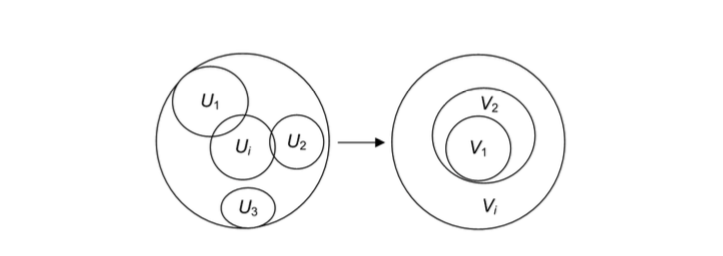
\includegraphics[scale=0.5]{2_1.png}
    \caption{ \textit{Một hướng cải tiến tiêu chuẩn kiểm định mã Sardinas-Patterson} }
\end{figure}
\begin{flushleft}
\hspace{10mm}Tính đúng đắn của thủ tục dựa trên Định lý \hyperlink{page.43}{\textcolor{blue}{2.1}} và các bổ đề sau đây.\\
\textbf{Bổ đề 2.1}      \textit{Cho $X \subseteq A^+$ và $V_i(i \ge 1)$ được định nghĩa theo công thức \hyperlink{page.42}{\textcolor{blue}{2.1}}Khi đó, với $z \in A^*$ tuỳ ý, $k \ge 1$, nếu $z \in V_k$ thì tồn tại $n,m \ge 1, x_1,x_2,...,x_n, y_1, y_2,...,y_m \in X$ sao cho}.
\end{flushleft}
$x_1x_2...x_n z = y_1y_2...y_m$ với $x_1 \ne y_1$.
\begin{flushleft}
\textit{Chứng minh}. Ta chứng minh quy nạp theo $k$ khẳng định trên.\\
\hspace{10mm} Với $k = 1$, giả sử $z \in V_1$ ta phải chứng minh tồn tại $n,m \ge 1, x_1, x_2, ..., x_n, y_1, y_2, ...,y_m \in X$, sao cho $x_1x_2...x_nz = y_1y_2...y_m$ với $x_1 \ne y_1$.\\
\hspace{10mm}Từ định nghĩa $V_1 = X^{-1}X - \{ \varepsilon \}, z\in V_1$, suy ra $z \in X^{-1}X = \{ \varepsilon \}$, nghĩa là tồn tại $x_1, y_1 \in X$ sao cho $x_1z \ y_1$. vì $\varepsilon \not\in V_1$ suy ra $x_1 \ne y_1$. \\
\hspace{10mm}Vậy, điều khẳng định đúng với k = 1.\\
\hspace{10mm}Giả sử điều khẳng định đã đúng với $k > 1$, ta chứng minh nó cũng đúng với trường hợp $k + 1$.\\
\hspace{10mm}Giả sử $z \in V_{k+1}$, ta phải chứng minh tồn tại $n,m \ge 1, x_1, x_2, ... , x_n, y_1, y_2,...,y_m \in X$ sao cho $x_1x_2...x_n z = y_1y_2...y_m$với $x_1 \ne y_1$.\\
\hspace{10mm}Theo định nghĩa $V_{k+1} = V^{-1}X \cup X^{-1}V_k \cup V_k$. Khi đó, từ $z \in V_{k+1}$, suy ra $z \in V_k$ (trường hợp 1) hoặc $z \in V_k^{-1}X$ (trường hợp 2) hoặc $z \in X^{-1}V_k$ (trường hợp 3). Ta xét các trường hợp sau.\\
\hspace{10mm}Trường hợp 1: $z \in V_k$. Theo giả thiết quy nạp, điều khẳng định đúng.
\hspace{10mm}Trường hợp 2: $z \in V^{-1}X$. Tồn tại $z' \in V_k$, theo giả thiết quy nạp, tồn tại $l,s \ge 1,x_1,x_2,...,x_l, y_1, y_2,...,y_s \in X$ sao cho
\end{flushleft}
$x_1x_2...x_1 z' = y_1y_2...y_s$ với $x_1 \ne y_1$.
\begin{flushleft}
Nhân $z$ vào hai vế của biểu thức trên, ta có
\end{flushleft}
$x_1_2...x_l z' z = y_1y_2...y_s z$ với $x_1 \ne y_1$.
\begin{flushleft}
Thay $z'z = x$ vào biểu thức trên ta nhận được
\end{flushleft}
$x_1x_2...x_lx = y_1y_2....y_sz$ với $x_1 \ne y_2$ 



\chapter{Phương pháp phân rã Dantzig-Wolfe giải bài toán kích thước lớn}
%%%%%%%%%%%%%%%%%%%%%%%%%%%%%%%%%%%%%%%%%%

Phương pháp phân rã Dantzig - Wofle là sự kết hợp giữa ý tưởng về việc giải quyết một bài toán QHTT tổng quát do Philip Wolfe đề xuất và phương pháp phân rã của Dantzig. Do vậy, để xem xét tận gốc của vấn đề, trước hết cần trình bày lại bài toán QHTT tổng quát của Wolfe.
%%%%%%%%%%%%%%%%%%%%%%%%%%%%%%%%%%%%%%%%%%
%+ Bai 2.1. Bai toan QHTT Wolfe tong quat
\section{Bài toán quy hoạch tuyến tính Wolfe tổng quát}

%+ 2.1.1. Phat bieu bai toan
\subsection{Phát biểu bài toán và các tính chất}
Xuất phát từ những bài toán ứng dụng thực tế, các hệ số $A, b$ và $c$ của bài toán QHTT \eqref{eq.2.1.1} thường thay đổi trong một tập nào đó. Điều này cho phép việc ứng dụng vào thực tế trở nên mềm dẻo hơn, phù hợp với ứng dụng thực tế hơn. Khi các hệ số $A, b, c$ thay đổi trong các tập lồi, bài toán này trở thành bài toán QHTT tổng quát được Philip Wolfe đề xuất. 

Bài toán QHTT Wolfe tổng quát được phát biểu như sau:
\begin{align}\label{eq.2.1.1}
&\min\set{f(x) = c^Tx}\\
&\text{thỏa mãn } D := \begin{cases}
Ax=b\\
x\geq 0\\
\end{cases}\notag
\end{align}
trong đó các hệ số $\binom{c_j}{A_j}\in C_j$ với mọi $j=1,\dots, n$. Ở đây, $C_j$ là các tập lồi nào đó trong $\R^{m+1}$ và $A_j$ là véc tơ cột thứ $j$ của ma trận $A$. Tổng quát hơn, người ta cũng có thể xem xét bài toán (\ref{eq.2.1.1}) với hệ số $b_i$ thay đổi, tức $b\in C_b$ nào đó với $C_b$ là tập lồi trong $\R^m$.

Vì các véc tơ $\binom{c_j}{A_j}$ chọn tùy ý trong các tập $C_j$, nên theo định lý biểu diễn tập lồi, với mỗi $j$, véc tơ $\binom{c_j}{A_j}$ có thể biểu diễn qua tập đỉnh và tập hướng cực biên của $C_j$. Trước hết ta sẽ chứng minh một định lý tổng quát cho bài toán Wolfe tổng quát.

%+ Dinh ly 2.1.1
\begin{theorem}\label{th.2.1.1}
Bài toán QHTT Wolfe tổng quát \eqref{eq.2.1.1} là tương đương với bài toán QHTT Wolfe tổng quát sau:
\begin{align}\label{eq.2.1.2}
&\min\set{\hat f(x,x^t) := \sum_{j=1}^n(c_jx_j + \sum_{t=1}^{T_j}c^t_jx_j^t)}\\
&\text{thỏa mãn } D := \begin{cases}
\sum_{j=1}^n(a_{ij}x_j + \sum_{t=1}^{T_j}a^t_{ij}x^t_j) = b_i,\\
x_j \geq 0,\quad i=1,\dots, m,\; j=1,\dots, n.
\end{cases}\notag
\end{align}
trong đó $\binom{c_j}{A_j}$ chọn tùy ý trong $C_j$ và $\binom{c^t_j}{A^t_j}$ là $T_j$ các điểm cố định trong $C_j$.
\end{theorem}
Chú ý rằng bài toán \eqref{eq.2.1.2} có số biến nhiều hơn bài toán \eqref{eq.2.1.1}. Do vậy tính tương đương ở đây thể hiện theo nghĩa, tập nghiệm của hai bài toán có thể suy ra nhau và giá trị hàm mục tiêu là bằng nhau.

%+ Chung minh.
\noindent{\it Chứng minh. }
Giả sử $x_j=x^{*}_j$ và $\binom{c_j}{A_j} = \binom{c^{*}_j}{A^{*}_j}$ với $j=1,\dots, n$ là nghiệm tối ưu của bài toán \eqref{eq.2.1.1} với giá trị $f(x^{*}) = f^{*}$ và giả sử $x_j=\hat x_j, x^t_j=\hat x_j^t$ và $\binom{c_j}{A_j} = \binom{\hat c_j}{\hat A_j}, \binom{c^t_j}{A^t_j} = \binom{\hat c^t_j}{\hat A^t_j},$ với $j=1,\dots, n$ là nghiệm tối ưu của bài toán \eqref{eq.2.1.2} với giá trị hàm mục tiêu tối ưu $\hat f(\hat x) = \hat f$.\\
Dễ thấy $x_j=x_j^{*}, x_j^t=0$ là nghiệm chấp nhận của bài toán \eqref{eq.2.1.2} nên ta có $f^{*}\leq \hat f$. 
Mặt khác, nghiệm tối ưu của bài toán \eqref{eq.2.1.2} có thể viết lại như là nghiệm chấp nhận của bài toán \eqref{eq.2.1.1} dưới dạng:
\begin{align*}
&\min\set{\sum_{j=1}^n\bar c_j\bar x_j}\\
&\text{thỏa mãn } \begin{cases}
\sum_{j=1}^n\bar a_{ij}\bar x_j = b_i,\quad i=1,\dots, m,\\
\bar x_j \geq 0, \quad j=1,\dots, n,
\end{cases}
\end{align*}
trong đó
\begin{align*}
&\bar x_j = \hat x_j + \sum_{t=1}^{T_j}\bar x^t_j,\\
&\binom{\bar c_j}{\bar A_j}= \begin{cases}
\binom{\hat c_j}{\hat A_j}\frac{\hat x_j}{\bar x_j} + \binom{\hat c^t_j}{\hat A^t_j}\frac{\bar x^t_j}{\bar x_j} \quad\text{với $\bar x_j\neq 0$},\\
\binom{\hat c_j}{\hat A_j} \quad\text{với $\bar x_j =  0$}.
\end{cases}
\end{align*}
Điều này có nghĩa là $\bar f \leq f^{*}$. Do vậy $\bar f=f^{*}$.
\hfill $\square$
%+ Ket thuc Dinh ly 2.1.1

Bây giờ để đơn giản việc nghiên cứu, ta hạn chế một số các hệ số $\binom{c_j}{A_j}$ thay đổi trong các tập $C_j$ một số các hệ số khác cố định, trong trường hợp này $\abs{C_j} = 1$ (tập hợp chỉ gồm 1 điểm).
Giả sử ta xét bài toán QHTT tổng quát có dạng:
\begin{equation}\label{eq.2.1.3}
 \begin{array}{lllll}
\min\set{ &c^Tx+y_{0,n+1}x_{n+1}&=z}\\
&Ax+y_{\bullet n+1}x_{n+1}&=b,&&\\
&(x,x_{n+1})&=(x_1,x_2,\dots,x_{n+1})\geq0.
\end{array}.
\end{equation}
trong đó $A=(a_{ij})_{m\times n}$ và các hệ số $\binom{y_{0,n+1}}{y_{\bullet n+1}}\in C_{n+1}$ là tập đơn hình có dạng:
\begin{equation}\label{eq.2.1.4}
C_{n+1}=\{y_{i,n+1}| \sum_{i=0}^m\alpha_iy_{i,n+1}=1,y_{i,n+1}\geq0, \textrm{ với }i=0,\dots,m\}
\end{equation}
Khi đó sử dụng định lý biểu diễn tập lồi, ta sẽ biểu diễn mỗi điểm $u\in C_{n+1}$ qua tập đỉnh của nó
\begin{equation}\label{eq.2.1.5}
(u_0, u) = \sum_{i=0}^m\alpha_iy_{i,n+1}.
\end{equation}
Sau đó thay vào bài toán \eqref{eq.2.1.3} ta sẽ thu được một bài toán QHTT với $n+m+1$ biến $x, \alpha_0,\dots, \alpha_m$. 
Khi đó ta có định lý sau:

%+ Dinh ly 2.1.1.
\begin{theorem}\label{eq.2.1.2}
Bài toán QHTT tổng quát dạng (\ref{eq.2.1.3}) là tương đương với bài toán QHTT thông thường
\begin{equation}\label{eq.2.1.5}
\begin{array}{lllll}
\min\set{& c^Tx+u_0&=w}\\
&Ax+u&=b&\\
&\sum_{i=0}^m\alpha_iu_{i,n+1}&=x_{n+1}\\
&x_1,x_2,\dots,x_{n+1}\geq0,& u_0,u_1,\dots,u_m\geq0
\end{array}.
\end{equation}
trong đó $A=(a_{ij})_{m\times n}$ và $u_i=y_{i,n+1}x_{n+1}$ với giả thiết rằng phương án tối ưu cho \eqref{eq.2.1.5} có $x_{n+1}=x^\ast_{n+1}>0$
\end{theorem}

%+ Chung minh.
\begin{proof}
Ta sẽ chứng minh mỗi phương án tối ưu của \eqref{eq.2.1.3} tìm được một phương án tối ưu của \eqref{eq.2.1.5} và ngược lại. 
Trước hết ta sẽ chỉ ra phương án tối ưu của \eqref{eq.2.1.3} là chấp nhận được cho \eqref{eq.2.1.5}. Giả sử $x^{*}$, $y_{i, n+1}^{*}$ và $z^{*}$ là tối ưu cho bài toán \eqref{eq.1.2.3}. Đặt $z=z^\ast$, $x_j=x_j^\ast$, $j=1,\dots,n+1$ với $x_{n+1}^\ast\geq 0$, và $y_{i,n+1}=y_{i,n+1}^\ast$, $i=0,\dots,m$. Khi đó nó là một phương án tối ưu chấp nhận được cho \eqref{eq.2.1.5}. Thật vậy, giá trị $x_j=x_j^\ast$, $j=1,\dots,n+1$ và $u_i=y_{i,n+1}^\ast x_{n+1}^\ast$, $i=0,\dots,m+1$, rõ ràng là chấp nhận được cho \eqref{eq.2.1.3} nghĩa là:
\begin{equation}\label{2.1.5a}
\begin{array}{llllll}
\min\set{&c^Tx^\ast&+y_{0,n+1}^\ast x^\ast_{n+1}&&=w^\ast}\\
&Ax^\ast&&+y_{\bullet,n+1}^\ast x^\ast_{n+1}&=b,\\
&&&\sum_{i=0}^m\alpha_iy^\ast_{i,n+1}x_{n+1}&=x_{n+1}^\ast.
\end{array}
\end{equation}
Do đó ta có $z^\ast\geq w^\ast$. 
Tiếp theo giả sử rằng $w^\ast$ không tối ưu nhưng tồn tại tập các giá trị $w=\overline{w},x_j=\overline{x_j}$ $j=1,\dots,m+1$ và $u_i=\overline{u_i}$, $i=0,\dots,m+1$ tập này là tối ưu chấp nhận được cho \eqref{eq.2.1.5}. Vì $\overline x_{n+1}>0$ theo giả thiết, ta tính $\overline y_{i,n+1}=\overline u_{n+1}/\overline x_{n+1}$ với $i=0,\dots,m$. Phương án $x_j=\overline x_j$, $j=1,\dots,n+1$ với $y_{i,n+1}=\overline y_{i,n+1}$, $i=0,\dots,m$ rõ ràng là chấp nhận được cho \eqref{eq.2.1.3} và vì vậy $\overline{w}\leq \overline{z}$. Do đó phương án tối ưu hai bài toán là tương đương. 
\end{proof}
%+ Ket thuc Dinh ly 2.1.1

Tiếp theo, để minh họa cho phương pháp Wolfe giải bài toán QHTT dạng \eqref{eq.2.1.3}, ta xem xét ví dụ sau:

%+ Vi du 2.1.1
\noindent{\bf Ví dụ 2.1.1. }
Xét bài toán xác định bởi hệ phương trình (\ref{eq.2.1.6})
\begin{equation}\label{eq.2.1.6}
\begin{array}{llllll}
\min&\set{6x_1&+4x_2&+x_3&+y_{04}x_4 & :=z}\\
&x_1&+x_2&-4x_3&+y_{14}x_4&=5\\
&-x_1&+x_2&-x_3&+y_{24}x_4&=1\\
&x_1\geq 0&x_2\geq 0&x_3\geq 0&x_4\geq 0
\end{array}.
\end{equation} 
với các hệ số $y_{\bullet4}=(y_{04},y_{14},y_{24})$ với $y_{i4}\geq0$ không cố định được chọn tùy ý trong đơn hình
\begin{equation}\label{eq.2.1.7}
C_4=\{y_{\bullet4}|\quad 3y_{04}+y_{14}+2y_{24}=2\textrm{ với } y_{i4}\geq 0\quad i=0,1,2\}
\end{equation}
và các hệ số còn lại cố định.

Giả sử ta có một cơ sở xuất phát của các biến $(-z, x_1, x_2)$, phương án cơ sở chấp nhận được cho dưới dạng:
\begin{displaymath}
(-z)=-24,\quad x_1=2,\quad x_2=3,\quad x_3=x_4 = 0.
\end{displaymath}
Bây giờ sử dụng thuật toán đơn hình để kiểm tra xem phương án đã cho có tối ưu không, ta tìm các nhân tử Lagrange, tức các biến đối ngẫu $\pi$ ứng với phương án đã cho bằng việc giải phương trình $B^T\pi = c_B$, tức $\pi = (B^{-1})^Tc_j$ với $B$ là cơ sở ứng với phương án đã cho ở trên. Giải ra ta có $\pi=(5,-1)^T$ và tính các ước lượng $\bar c_3$ và $\bar c_4$ với $\overline{c_j}=c_j-\pi^TA_{\bullet j}$ ta thu được:
$$
\overline{c_3}=18, \;\overline{c_4}=y_{04}-5y_{14}+y_{24}
$$
tron đó $(y_{04},y_{14},y_{24})\in C_4$. 
Theo thuật toán đơn hình, nếu các ước lượng $\bar c_3, \bar c_4 \geq 0$ thì phương án đang xét là tối ưu. Trong trường hợp này vì $\bar c_3=20>0$ nên chỉ còn $c_4$ là phụ thuộc vào tập $C_4$. Để kiểm tra $\bar c_4$, ta tìm giá trị nhỏ nhất của $\bar c_4$ trên tập $C_4$ bằng việc giải bài toán QHTT:
\begin{equation}\label{eq.2.1.8}
\begin{array}{llllll}
\min &y_{04}&-5y_{14}&+y_{24}&=\overline{c_4}\\
&3y_{04}&+y_{14}&+2y_{24}&=2\\
&&y_{i4}\geq0 & i=0,1,2\\
\end{array}.
\end{equation}
Ta thu được $y_{04}=0$, $y_{14}=2$, $y_{24}=0$ và $\overline{c_4}=-10$. Do đó vẫn tồn tại điểm trong $C_4$ sao cho $\bar c_4 < 0$, tức phương án đang xét  
\begin{displaymath}
(-z)=-24,\quad x_1=2,\quad x_2=3,\quad x_3=x_4 = 0.
\end{displaymath}
chưa phải là phương án tối ưu cho bài toán \eqref{eq.2.1.6}.

Để cải thiện phương án của bài toán \eqref{eq.2.1.6}, ta đưa biến $x_4$ vào cơ sở và tìm một biến đưa ra khỏi cơ sở để có cơ sở mới. Trong trường hợp này, theo quy tắc của phương pháp đơn hình, biến $x_1$ sẽ đưa ra khỏi cơ sở, ta có cơ sở mới là $\set{2, 4}$ với giá trị
$$
(-z)=-4,\quad x_2=1,\quad x_4=2,\quad x_1=x_3=0
$$
Tuy nhiên để bảo toàn biến $y_{i4}$ thu được ở bước trước của thuật toán, thay vì xem xét bài toán \eqref{eq.2.1.6}, theo Định lý \ref{th.2.1.1}, ta xem xét bài toán tương đương với nó có dạng:

\begin{equation}\label{eq.2.1.9}
\begin{array}{lllllll}
&6x_1&+4x_2&+x_3&+0x^{(1)}_4&+y_{04}x_4&=z(\min)\\
&x_1&+x_2&-4x_3&+2x^{(1)}_4&+y_{14}x_4&=5\\
&-x_1&+x_2&-x_3&+0x_4&+y_{24}x_4&=1\\
&x_1\geq 0,&x_2\geq 0,&x_3\geq 0,&x_4\geq 0,&x^{(1)}_4\geq 0
\end{array}.
\end{equation} 
ở đây $y_{\bullet 4}\in C_4$.\\
Như ở trên, ta có phương án cơ sở cho bài toán \eqref{eq.2.1.9} là
\begin{displaymath}
(-z)=-4,\quad x_2=1,\quad x^{(1)}_4=2,\quad x_1=x_3=x_4=0
\end{displaymath}
và phương án đối ngẫu (hay nhân tử Lagrange) sẽ là $\pi = (0, 4)^T$. Khi đó các ước lượng cho hệ số sẽ là:
$$
\overline{c_1}=10, \quad \overline{c_3}=5,\quad \overline{c_4}=y_{04}-4y_{24}.
$$
Các giá trị $\overline{c_1},\overline{c_3}$ là không âm. Do vậy ta chỉ cần kiểm tra $c_4$. Để kiểm tra $c_4$ có nhỏ hơn 0 hay không ta giải bài toán QHTT phụ:
\begin{equation}\label{eq.2.1.10}
\begin{array}{llllll}
\min &y_{04}&&-4y_{24}&=\overline{c_4}\\
&3y_{04}&+y_{14}&+2y_{24}&=2\\
&y_{i4}\geq0 .
\end{array}.
\end{equation}
Bài toán này có cùng tập ràng buộc là đơn hình $C_4$ như bài toán phụ ở bước trước, chỉ khác nhau hàm mục tiêu. Giải bài toán \eqref{eq.2.1.10} ta thu được $\overline{c_4}=-4$, $y_{04}=0$, $y_{14}=0$, $y_{24}=1$. Do $\bar c_4=-4<0$ nên phương án 
\begin{displaymath}
\label{126}(-z)=-4,\quad x_2=1,\quad x^{(1)}_4=2,\quad x_1=x_3=x_4=0
\end{displaymath}
vẫn chưa tối ưu cho bài toán \eqref{eq.2.1.6}. Khi đó biến $x_4$ đưa vào cơ sở và loại bỏ $x_2$ ra khỏi cơ sở được phương án chấp nhận được mới là:
\begin{displaymath}
(-z)=-4,\quad x^{(1)}_4=\frac{5}{2},\quad x_4=1,\quad x_1=x_2=x_3=0
\end{displaymath}
Tiếp tục lập bài toán QHTT mới tương đương với \eqref{eq.2.1.6} mà $y_{i4}$ được xét lại:
\begin{equation}\label{eq.2.1.11}
\begin{array}{lllllllll}
&6x_1&+4x_2&+x_3&+0x^{(1)}_4&+0x^{(2)}_4&+y_{04}x_4&=z(\min)\\
&x_1&+x_2&-4x_3&+2x^{(1)}_4&+0x^{(2)}_4&+y_{14}x_4&=5\\
&-x_1&+x_2&-x_3&+0x_4^{(1)}&+1x^{(2)}_4&+y_{24}x_4&=1\\
&x_1\geq0,&x_2\geq0,&x_3\geq0,&x_4\geq0,&x^{(1)}_4\geq0,&x^{(2)}_4\geq0.
\end{array}.
\end{equation} 
Phương án cơ sở chấp nhận được mới là:
\begin{displaymath}
(-z)=0,\quad x^{(1)}_4=-\frac{5}{2},\quad x^{(2)}_4=1, \quad x_1=x_2=x_3=x_4=0
\end{displaymath}
Tương ứng với nó là phương án đối ngẫu (hay nhân tử Lagrange) thu được sẽ là $\pi=(0,0)^T$ và các ước lượng tính được là $\overline{c_1}=6$, $\overline{c_2}=4$, $\overline{c_3}=1$, $\overline{c_4}=y_{04}$. 
Tiếp theo để kiểm tra $\overline{c_4}=y_{04}$, ta giải bài toán phụ:
\begin{equation}\label{eq.2.1.12}
\begin{array}{lllll}
\min &y_{04}&=\overline{c_4}\\
&3y_{04}+y_{14}+y_{24}&=2\\
&y_{i4}\geq0\end{array} .
\end{equation}
Giải bài toán này ta thu được $\overline{c_4}=0$, $y_{04}=0$, $y_{14}=2$, $y_{24}=0$. Vì tất cả các ước lượng của bài toán \eqref{eq.2.1.11} đều không âm cho mọi giá trị của $y_{\bullet4}$ nên phương án đang xét là tối ưu cho \eqref{eq.2.1.11}. Để khôi phục lại nghiệm bài toán gốc \eqref{eq.2.1.6} ta thấy rằng:
\begin{displaymath}
z=0,\quad x_1=x_2=x_3=0,\quad x_4=x^{(1)}_4=x^{(2)}_4=\frac{7}{2}
\end{displaymath}
và tính được:
\begin{displaymath}
\left (\begin{matrix}y_{04}\\y_{14}\\y_{24}\end{matrix}\right )=y^{(1)}_{\bullet4}\frac{x^{(1)}_4}{x^{(1)}_4+x^{(2)}_4}+y^{(2)}_{\bullet4}\frac{x^{(2)}_4}{x^{(1)}_4+x^{(2)}_4}=\left(\begin{matrix}0\\2\\0\end{matrix}\right).\frac{5}{7}+\left(\begin{matrix}0\\0\\1\end{matrix}\right).\frac{2}{7}=\left(\begin{matrix}0\\10/7\\2/7\end{matrix}\right).
\end{displaymath}
%+ Ket thuc Vi du 2.1.1.

%+ --------------------------------------------------------------------------------------------------
\subsection{Trường hợp bài toán phụ có phương án không bị chặn. }
Chú ý rằng, trong phương pháp Wolfe, ta cần phải giải liên tiếp các bài toán QHTT phụ trên tập ràng buộc $C_j$. Có thể xảy ra trường hợp tập ràng buộc này không bị chặn, và khi đó bài toán phụ có thể không bị chặn dưới. Khi giải bài toán phụ, sẽ có hai trường hợp:
\begin{itemize}
\item [$1)$] Nếu một phương án cực biên $y_{\bullet s}=y^e_{\bullet s}\in C_s$ thu được với $y^e_{\bullet s}$ là điểm cực biên, thì nếu cước phí $\bar c_s$ là âm thì đưa nó vào cơ sở của bài toán gốc.
\item [$2)$] Nếu một lớp các phương án $y_{\bullet s}=y^e_{\bullet s}+\theta y^h_{\bullet s}\in C_s$ với $y^e_{\bullet s}$ là điểm cực biên, $y^h_{\bullet s}$ là các hướng cực biên, với $\theta$ là một tham số vô hướng. Thì chỉ cần đưa các hướng cực biên $y^h_{\bullet s}$ vào cơ sở của bài toán gốc. Cơ sở cho việc xử lý này là ta viết lại $y_{\bullet s}x_s$ như sau:
\begin{displaymath}
y_{\bullet s}x_s=(y^e_{\bullet s}+\theta y^h_{\bullet s})x_s=(
\frac{1}{\theta} y^e_{\bullet s}+y^h_{\bullet s})\theta x_s
\end{displaymath}.
Thì do $\theta>0$ tùy ý, nên hướng cực biên này sẽ làm cho giá trị của mục tiêu $\bar c_s$ giảm tới mức âm. 
\end{itemize}

%%%%%%%%%%%%%%%%%%%%%%%%%%%%%%%%%%%%%%%%%%%
%+ Bai 2.2. Nguyen ly phan ra Dantzig-Wolfe
\section{Nguyên lý phân rã Dantzig-Wolfe(D-W)}

Nguyên lý phân rã Dantzig-Wolfe dựa trên định lý biểu diễn tập lồi đa diện. Ta đã biết rằng, trong giải tích lồi, một tập lồi đa diện $P$ có số điểm cực biên $V(P)$ và số hướng cực biên $E(P)$ là hữu hạn, và mọi điểm $x$ trong tập lồi đa diện $P$ đều có thể biểu diễn qua tổ hợp lồi các điểm cực biên và tổ hợp không âm các hướng cực biên của nó, nghĩa là:
\begin{equation}\label{eq.2.2.1}
x = \sum_{v^i\in V(C)}\alpha_iv^i + \sum_{e^j\in E(C)}\beta_je^j,
\end{equation}
trong đó $\alpha_i, \beta_j\geq 0$ và $\sum_{i}\alpha_i = 1$.\\
Đối với tập lồi đa diện $P$ có dạng:
\begin{equation}\label{eq.2.2.2}
P :=\set{x\in \R^n\;|\; Ax=b, x\geq 0}
\end{equation}
thì tập hợp các hướng vô hạn của $P$ sẽ là $Ay=0, y\geq 0$. Do đó ta định nghĩa hướng cực biên chuẩn hóa như sau:
%+ Dinh nghia 2.2.1
\begin{definition}
Các hướng cực biên chuẩn hóa của tập lồi đa diện $P$ cho bởi \eqref{eq.2.2.2} sẽ là các nghiệm cơ sở của hệ phương trình:
\begin{equation}\label{eq.2.2.3}
\left\{ \begin{array}{l}
Ay = 0\\
e^Ty = 1\\
y \geq 0
\end{array} \right .
\end{equation}
với $e^T = (1, 1,\ldots, 1)^T$ (véc tơ các thành phần đều là $1$).
\end{definition}
Chú ý rằng, nếu $\text{A}=m<n$ thì số nghiệm cơ sở (hay số nghiệm độc lập tuyến tính) của hệ này là $n-m$ và thỏa mãn điều kiện không âm và có tổng các thành phần bằng $1$.
Hiển nhiên số hướng cực biên chuẩn hóa luôn hữu hạn.

%+ 2.2.1. Y tuong cua phuong phap phan ra Dantzig - Wolfe.
\subsection{Ý tưởng của phương pháp phân rã Dantzig-Wolfe}
\noindent{\bf a. Ý tưởng chung. } Giả sử ta có một bài toán QHTT kích thước lớn với ràng buộc dạng $Ax=b, x\geq 0$. 
Phương pháp phân ra D-W thực hiện như sau:
\begin{itemize}
\item Ta sẽ phân rã ràng buộc này thành các ràng buộc dạng $A^kx=b^k$ với $k=1, \dots, p$ nào đó. Hiển nhiên nếu $A$ có dạng chéo khối với $p$ khối, ta có thể phân rã bài toán thành $p$ bài toán QHTT độc lập có kích thước nhỏ hơn. 
\item Khi $A$ có dạng tùy ý, ta có thể xem bài toán QHTT thỏa mãn ràng buộc $A^1x=b$ và thỏa mãn thêm ràng buộc $A^kx=b^k$ với $k=2,\dots, p$ và $x\geq 0$. Ta xem các ràng buộc thêm này như một tập lồi đa diện, và các điểm trong đó thỏa mãn định lý biểu diễn tập lồi. 
\item Biểu diễn biến $x$ qua các điểm cực biên và hướng cực biên chuẩn hóa của tập lồi da diện cần thỏa mãn.
\item Thay $x$ vào bài toán chỉ có ràng buộc $A^1x=b^1$, thu được bài toán với các biến mới $\alpha_i,\beta_j$.
\item Hạn chế số đỉnh, số hướng cực biên chuẩn hóa, giải quyết bài toán hạn chế. Nếu thỏa mãn điều kiện tối ưu cho bài toán ban đầu dừng lại. Ngược lại, thêm một đỉnh mới hoặc hướng cực biên chuẩn hóa mới và lặp lại việc giải bài toán đó.
\end{itemize}
Chú ý rằng, để tăng hiệu quả của phương pháp phân rã D-W, điều quan trọng là khai thác cấu trúc của ma trận ràng buộc. Tùy thuộc vào cấu trúc của ma trận $A$ mà người ta lựa chọn cách phân rã bài toán một cách hợp lý nhằm giảm tối đa kích thước bài toán con và bài toán con được giải quyết hiệu quả. Thậm chí trong trường hợp ma trận là chéo khối, thì việc giải bài toán con có thể làm một cách độc lập, song song trên các máy tính khác nhau.

%+ b. Noi dung phuong phap.
\noindent{\bf b. Nội dung phương pháp phân rã Dantzig - Wolfe. } 
Để đơn giản cách trình bày, ta xét bài toán QHTT chuẩn tắc dạng
\begin{equation}\label{eq.2.2.4}
 \begin{array}{llll}
\min\set{& c^Tx &= z}\\
&Ax &= b &\\
&x \geq 0,
\end{array} .
\end{equation}
trong đó $A$ là ma trận cỡ $m\times n$.
Trước hết, ta phân rã tập $D:= \set{Ax=b, x\geq 0}$ bởi hai phần $A^1x = b^1$ và $A^2x = b^2, x\geq 0$ với $A^1, A_2$ là các ma trận cỡ $m_1\times n$ và $m_2\times n$, tương ứng. Bài toán \eqref{eq.2.2.4} trở thành
\begin{equation}\label{eq.2.2.5}
 \begin{array}{llll}
\min\set{&c^Tx &= z}\\
&A^1x &= b^1 &\\
&A^2x &= b^2 &\\
&x \geq 0.
\end{array}.
\end{equation}
Hay, ta có thể viết lại như sau
\begin{equation}\label{eq.2.2.6}
 \begin{array}{llll}
\min\set{&c^Tx &= z}\\
&A^1x& = b^1&\\
&x \geq 0
\end{array}  .
\end{equation}
thỏa mãn thêm ràng buộc
\begin{equation}\label{eq.2.2.7}
P := \left\{ \begin{array}{lll}
A^2x = b^2&\\
x \geq 0
\end{array} \right .
\end{equation}
Hiển nhiên $P$ là một tập lồi đa diện chính tắc, ta gọi số đỉnh của $P$ là $V(P):=\set{u^i\:\; i=1,\dots, L}$ và số hướng cực biên chuẩn hóa của $P$ à $E(P):=\set{v^j\;|\; j=1, \dots, M}$. Khi đó, theo định lý biểu diễn tập lồi (Định lý \ref{th.1.1.1}) mọi điểm trong $P$ đều có thể biểu diễn dưới dạng:
\begin{equation}\label{eq.2.2.8}
x = \sum_{i=1}^L\alpha_iv^i + \sum_{j=1}^M\beta_je^j,
\end{equation}
trong đó $\alpha_i, \beta_j\geq 0$ và $\sum_{i=1}^L\alpha_i = 1$ với $i=1,\dots, L, j=1,\dots, M$.
Thay vào \eqref{eq.2.2.6} ta thu được bài toán có dạng:
\begin{equation}\label{eq.2.2.9}
 \begin{array}{ll}
\min \set{\sum_{i = 1}^L (c^Tu^i)\alpha_i + \sum_{j = 1}^M (c^Tv^j)\beta_j & =z},\\
\sum_{i = 1}^L (A^1u^i)\alpha_i + \sum_{j = 1}^M (A^1v^j)\beta_j & =b^1,\\
\sum_{i = 1}^L \alpha_i &= 1,\\
\alpha_i \geq 0, \quad i = 1, \ldots, L,\\
\beta_j \geq 0, \quad j = 1, \ldots, M.
\end{array} .
\end{equation}
Bằng cách đặt
\begin{align}\label{eq.2.2.10}
G^i &= A^1u^i, &H^j &= A^1v^j,\\
g_i &= c^Tu^i, &h_j &= c^Tv^j.\notag
\end{align}
Bài toán \eqref{eq.2.2.9} được viết gọn dưới dạng:
\begin{equation}\label{eq.2.2.11}
 \begin{array}{llll}
\min\set{\sum_{i = 1}^L g_i\alpha_i + \sum_{j = 1}^M h_j\beta_j & =z},\\
\sum_{i = 1}^L G^i \alpha_i + \sum_{j = 1}^M H^j \beta_j & = b^1 & :\pi,\\
\sum_{i = 1}^L \alpha_i & = 1 & :\gamma,\\
\alpha_i \geq 0,\quad i = 1, \ldots, L,\\
\beta_j \geq 0, \quad j = 1, \ldots, M.
\end{array}.
\end{equation}
Bài toán \eqref{eq.2.2.11} là một bài toán QHTT theo các biến $\alpha_i$ và $\beta_j$ với $i=1,\dots, L$, $j=1,\dots, M$. Bài toán \eqref{eq.2.2.11} được gọi là bài toán {\bf Full Master Program}. Rõ ràng, nếu số đỉnh $V(P)$ và số hướng cực biên $E(P)$ của tập $P$ là lớn thì bài toán \eqref{eq.2.2.11} sẽ có kích thước lớn. Ở đây $\pi\in \R^{m_1}$ và $\gamma \in R$ là các biến đối ngẫu (hay nhân tử Lagrange) tương ứng với các ràng buộc của bài toán \eqref{eq.2.2.11}.

%+ Dinh nghia 2.2.1.
\begin{definition}\label{de.2.2.1}
Hai bài toán QHTT \eqref{eq.2.2.4} và \eqref{eq.2.2.11} được gọi là tương đương, nếu $x$ là phương án chấp nhận của bài toán \eqref{eq.2.2.4} thì tồn tại $\alpha_i$ và $\beta_j$ với $i=1,\dots, L$, $j=1,\dots, M$ là phương án chấp nhận của bài toán \eqref{eq.2.2.11} sao cho
$$
x = \sum_{i=1}^L\alpha_iu^i + \sum_{j=1}^M\beta_jv^j
$$
và ngược lại.
\end{definition}
Với cách định nghĩa hai bài toán tương đương như định nghĩa \ref{de.2.2.1}, ta có định lý sau:
%+ Dinh ly 2.2.1
\begin{theorem}\label{th.2.2.1}
Bài toán QHTT chính tắc \eqref{eq.2.2.4} là tương đương với bài toán QHTT {\bf Full Master Program} \eqref{eq.2.2.11} theo nghĩa tương đương được định nghĩa như trong định nghĩa \ref{de.2.2.1}.
\end{theorem}
Hiển nhiên định lý này cũng cho ta biết, nếu $x^{*}$ là phương án tối ưu của \eqref{eq.2.2.4} thì tồn tại $\alpha_i^{*}$ và $\beta_j^{*}$ với $i=1,\dots, L$, $j=1,\dots, M$ là phương án tối ưu của bài toán \eqref{eq.2.2.11} sao cho
$$
x^{*} = \sum_{i=1}^L\alpha_i^{*}u^i + \sum_{j=1}^M\beta_j^{*}v^j
$$
và ngược lại. 

Thuật toán phân rã D-W không giải trực tiếp bài toán {\bf Full Master Program} \eqref{eq.2.2.11} mà giải trên bài toán hạn chế sẽ được định nghĩa dưới đây.
Ta gọi 
$$
L_{\max} := \set{1,2,\dots, L},\quad M_{\max} := \set{1,2,\dots, M},
$$
và $\bar M, \bar L$ là những tập con của $M_{\max}$ và $L_{\max}$ tương ứng. Khi đó ta định nghĩa.
%+ Dinh nghia 2.2.2
\begin{definition}\label{de.2.2.2}\textbf{Restricted Master Program}\\
Bài toán thu được từ \eqref{eq.2.2.11} bằng cách hạn chế các tập định của $P$ trên tập $\overline M$ và hạn chế các hướng cực biên của $P$ trên $\overline L$ gọi là bài toán {\bf Restricted Master Program}, nghĩa là:
\begin{equation}\label{eq.2.2.12}
 \begin{array}{llll}
\min\set{\sum_{i \in\bar L} g_i\alpha_i + \sum_{j \in\bar M} h_j\beta_j & =z&},\\
\sum_{i\in\bar L}G^i\alpha_i + \sum_{j \in\bar M} H^j\beta_j & =b^1&:\pi,\\
\sum_{i = 1}^L \alpha_i &= 1&:\gamma,\\
\alpha_i \geq 0, \quad i \in L,\\
\beta_j \geq 0, \quad j\in M.
\end{array}.
\end{equation}
\end{definition}
Câu hỏi tiếp theo là từ nghiệm bài toán hạn chế \eqref{eq.2.2.12} làm thế nào để kiểm tra xem đã là tối ưu cho bài toán cần giải chưa? Để trả lời câu hỏi này, ta xuất phát từ tiêu chuẩn tối ưu trong phương pháp đơn hình. Chú ý rằng, bài toán {\bf Full Master Program} và bài toán hạn chế \eqref{eq.2.2.12} đều là các bài toán QHTT chính tắc. 

Nếu ta ký hiệu $(\bar \pi,\bar\gamma)$ là phương án cơ sở đối ngẫu thì, thì nó sẽ thỏa mãn hệ ràng buộc đối ngẫu dạng:
\begin{equation}\label{eq.2.2.13}
\left\{ \begin{array}{lll}
\gamma + (G^i)^T \pi &= g_i, &i = 1,2, \ldots, k\\
        (H^j)^T \pi &= h_j, &j = 1,2, \ldots, l.
\end{array} \right .
\end{equation}
Phương pháp đơn hình sẽ chọn véc tơ mới đưa vào cơ sở dựa trên quy tắc là cho hàm mục tiêu giảm nhiều nhất, nghĩa là, ta chọn chỉ số $i=i^{*}$ và $j=j^{*}$ từ điều kiện:
\begin{equation}\label{eq.2.2.14}
g_{i^\ast} - (G^{i^\ast})^T \overline \pi - \overline \gamma = \min_{i = 1, \ldots, L} \{ g_i - (G^i)^T \overline \pi \} - \overline \gamma
\end{equation}
và
\begin{equation}\label{eq.2.2.15}
h_{j^\ast} - (H^{j^\ast})^T \overline \pi = \min_{j = 1, \ldots, M} \{ h_j - (H^j)^T \overline \pi \}
\end{equation}
Khi đó véc tơ cột của ma trận ràng buộc ứng với chỉ số $(i^{*}, j^{*})$ sẽ được đưa vào cơ sở. Ta định nghĩa độ lệch đối ngẫu bởi:
\begin{equation}\label{eq.2.2.16}
\bar\rho  = c - (A^1)^T \overline \pi
\end{equation}
và thay thế $G^i = A^1u^i$ và $H^j = A^1v^j$ để thu được:
\begin{align}\label{eq.2.2.17}
\min_{i = 1, \ldots, L} \{g_i - (G^i)^T \overline \pi \} - \overline \gamma
            &= \min_{i = 1, \ldots, L} \{ c^Tu^i - (A^1u^i)^T \overline \pi \} - \overline \gamma\notag\\
            &= \min_{i = 1, \ldots, L} \{ (c^T - (A^1)\overline \pi)^Tu^i \} - \overline \gamma\notag\\
            &= \min_{i = 1, \ldots, L} \{ \overline \rho^T u^i \} - \overline \gamma\notag.
\end{align}
Tương tự
\begin{equation}\label{eq.2.2.18}
\min_{j = 1, \ldots, M} \{h_j - (H^j)^T \overline \pi \} = \min_{j = 1, \ldots, M} \{ \overline \rho^T v^j \} 
\end{equation}
Đến đây ta vẫn chưa biết có điểm cực biên hai hướng cực biên chuẩn hóa nào mà có giá âm. Để xác định xem \eqref{eq.2.2.16} có giá âm hay không, ta không phải đi ước lượng trên toàn bộ số đỉnh của $P$ mà thay vào đó, ta giải một bài toán QHTT dạng:
\begin{equation}\label{eq.2.2.18}
 \begin{array}{ll}
\min\set{ \overline \rho^Tx &= z_2 + \overline \gamma}\\
A^2x &= b^2\\
x \geq 0
\end{array}  .
\end{equation}
với $\overline \rho = c - (A^1)^T \overline \pi$ thỏa mãn \eqref{eq.2.2.16} và $\overline \gamma$ là biến đối ngẫu ứng với ràng buộc lồi của bài toán {\bf Restricted Master Program} để xác định nghiệm $x=u^{*}$ là điểm cực biên của $P$.

Sau khi sử dụng phương pháp đơn hình mà phương án tối ưu là một phương án cơ sở chấp nhận $x = u^\ast$, thì ta tìm được cột với cước phí thu gọn nhỏ nhất cho bài toán {\bf Full Master Program}. Nếu $u^\ast$ là tối ưu, và nếu $\min z_2 \leq 0$ ta bổ sung vào cho bài toán {\bf Restricted Master Program} thêm cột mới bởi
\begin{equation}\label{eq.2.2.19}
\begin{pmatrix}
G^\ast\\
g^\ast\\
1
\end{pmatrix}
=
\begin{pmatrix}
A^1u^\ast\\
c^Tu^\ast\\
1
\end{pmatrix}
\end{equation}
với chỉ số $\ast$ nhằm thể hiện việc đánh số lại các chỉ số cho phù hợp với bài toán {\bf Restricted Master Progam} mới thu được. Tiếp theo lại tối ưu lại bài toán hạn chế thu được này. Nếu $\min z_2 = 0$ thì tất cả cước phí thu gọn với bài toán Full Master Program \eqref{eq.2.2.11} không âm. Trong trong trường hợp này từ phương án tối ưu của bài toán Full Master Program và \eqref{eq.2.2.8} có thể tìm được phương án tối ưu cho bài toán ban đầu \eqref{eq.2.2.4}.

Trong trường hợp còn lại, giả sử giải bài toán \eqref{eq.2.2.18}) bằng phương pháp đơn hình cho ta một phương án cực biên thuần nhất $x^h = v^\ast$. Trong trường hợp này, theo lý thuyết, ta không cần ước lượng tất cả các hướng cực biên chuẩn hóa \eqref{eq.2.2.7} mà có thể tìm được hướng cực biên tốt nhất bằng cách giải bài toán QHTT:
\begin{equation}\label{eq.2.2.20}
 \begin{array}{ll}
\min\set{ \overline \rho^Tx &= z_2^h}\\
A^2x &= 0\\
e^Tx &= 1\\
x \geq 0
\end{array}  .
\end{equation}
với $e=(1,\dots,1)^T$, $\overline\rho$ thỏa mãn \eqref{eq.2.2.16} và $z_2^h$ là giá trị tối ưu tương ứng với nghiệm của nó. Tuy nhiên, việc giải quyết bài toán này sẽ là không cần thiết vì sẽ tăng chi phí tính toán cho thuật toán. Trên thực tế, ta chỉ cần chọn một hướng cực biên chuẩn hóa $x^h=v^\ast$ nào đó của \eqref{eq.2.2.7} mà làm cho ước lượng véc tơ giá là âm. Khi đó ta đưa cột 
\begin{equation}\label{eq.2.2.21}
\begin{pmatrix}
H^\ast\\
h^\ast\\
0
\end{pmatrix}
=
\begin{pmatrix}
A^1v^\ast\\
c^Tv^\ast\\
0
\end{pmatrix}
\end{equation}
vào cơ sở của bài toán thu gọn để thu được bài toán mới và giải lại bài toán này.

%+ Chu ý 2.2.1.
\begin{remark}
Trong thủ tục đơn hình, để tính các ước lượng của các véc tơ $A_k$, gọi là $\Delta_k = \sum_{j\in J}z_{jk}c_j - c_k$. Nếu $\Delta_k\leq 0$ với mọi $k$ thì phương án đang xét là tối ưu. Đây chính là tiêu chuẩn tối ưu của thuật toán đơn hình mà ta đã sử dụng trong thuật toán này. Trên thực tế, ta không tính các ước lượng này thông qua các hệ số $z_{jk}$ mà thông qua các biến đối ngẫu $\pi, \gamma$ như công thức đề cập trong chương 1.
\end{remark}

%+2.2.2. Thuat toan D-W
\subsection{Thuật toán Dantzig-Wolfe và phương án xuất phát}
%+ Thuat toan 
\textbf{a. Thuật toán Dantzig-Wolfe. } Thuật toán phân rã Dantzig - Wolfe được mô tả như sau:\\
\noindent{\it Đầu vào: } Dữ liệu của bài toán QHTT: Véc tơ giá $c$, Ma trận ràng buộc $A^1$ véc tơ vế phải $b^1$, tập lồi đa diện $P$ với tập đỉnh $\bar L$ và tập hướng cực biên $\bar L$ xuất phát cho bài toán {\it Restricted Master Program}.\\
\noindent{\it Đầu ra: } Khẳng định bài toán \eqref{eq.2.2.4} vô nghiệm hoặc tìm được một nghiệm tối ưu $x^{*}$.\\
\noindent{\it Thuật toán: }
\begin{itemize}
\item[$1.$ ] Từ bài toán {\it Restricted Master Program} với một phương án cơ sở chấp nhận được xuất phát và một cột không cơ sở.
\item[$2.$ ] Giải bài toán {\it Restricted Master Program}. Nếu tìm được một nghiệm tối ưu thì đi đến bước 3 nếu khác thông báo bài toán gốc không bị chặn và dừng.
\item[$3.$ ] Nghiệm cơ sở chấp nhận được tối ưu của bài toán Restricted Master Program cùng với nhân tử đơn hình $\binom{\overline\pi}{\overline\gamma}$ giúp ta loại ra cột không cơ sở.
\item[$4.$ ] Giải bài toán con \eqref{eq.2.2.18}.
\item[$5.$ ] Nếu từ \eqref{eq.2.2.18} tìm được phương án cơ sở chấp nhận được tối ưu và $\min z_2 < 0 $ thì cột \eqref{eq.2.2.19} được thêm vào bài toán {\it Restricted Master Program} và quá trình tiếp tục ở bước 2.
\item[$6.$] Nếu từ \eqref{eq.2.2.18} ta thu được một hướng cực biên thuần nhất không âm thì cột \eqref{eq.2.2.21} được thêm vào bài toán {\it Restricted Master Program} quá trình tiếp tục ở bước 2.
\item[$7.$] Nếu $z_2=0$, từ phương án này tìm được phương án tối ưu cho bài toán gốc. Phương án tối ưu được cho bởi \eqref{eq.2.2.7} với $\alpha_1,\alpha_2,\dots$và $\beta_1,\beta_2,\beta_3,\dots$ là phương án tối ưu cho bài toán {\it Restricted Master Program} cuối cùng. Nó chính là phương án tối ưu chấp nhận được cho bài toán {\it Full Master Program}.
\end{itemize}
Chú ý rằng, một phương án cơ sở tối ưu của bài toán {\it Restricted Master Program} cũng là phương án tối ưu cơ sở cho bài toán{\it Full Master Program} nếu 
\begin{equation}\label{eq.2.2.22}
\min z_2 = \bar\gamma.
\end{equation}
Công thức này suy ra từ điều kiện \eqref{eq.2.2.18}. Khi đó độ lệch đối ngẫu $\bar\rho^Tx^{*} = 0$.\\
Bên cạnh đó, nếu bài toán QHTT \eqref{eq.2.2.4} là không suy biến thì thuật toán D-W sẽ dừng sau hữu hạn bước lặp. Hoặc tìm được phương án tối ưu hoặc chỉ ra một hướng cực biên mà hàm mục tiêu giảm ra $-\infty$.

%+ Tim phuong an xuat phat.
\textbf{b. Phương án xuất phát của thuật toán Dantzig-Wolfe. }\\
Trong phần này chúng ta sẽ trình bày phương pháp tìm phương án xuất phát của thuật toán Dantzig-Wolfe. Trước hết phải ta cần phải xác định một đỉnh của tập $P$ là $u^1$. Việc này có thể được làm bằng cách sử dụng Pha 1 của thuật toán đơn hình để giải bài toán phụ dạng.
\begin{equation}\label{eq.2.2.23}
\begin{array}{lll}
\min \quad \sum_{i=1}^{m_2}v_i = f(u, v)\\
\sum_{j=1}^na^2_{ij}u_j + v_i = b^2\\
u_j\geq 0, v_i\geq 0, i=1,\dots,m_1, j=1,\dots, n.
\end{array}
\end{equation}
Sau khi có một đỉnh $u^1$ của tập $P$, ta đặt $G^1=A^1u^1$ ta thiết lập bài toán {\it Restricted Master Program} với biến giả $\xi_i$.
\begin{equation}\label{PT030}
\begin{array}{lll}
\min \quad \sum_{i=1}^{m_1}\xi_i=w\\
G^1\alpha_1+\sum_{i=1}^{m_1}\pm e^i\xi_i=b^1\\
\alpha_1=1\\
\alpha_1\geq0,\quad \xi_i\geq0,\quad i=1,\dots,m_1
\end{array}
\end{equation}
trong đó $e^i$ là cột thứ $i$ của ma trận đơn vị $m_1\times m_1$ chú ý rằng $\alpha_1$ phải bằng 1. Do đó trong đẳng thức thứ 2 là $+e^i$ nếu $b^1_i-G^1_i\geq0$ và $-e^i$ nếu $b^1_i-G^1_i<0$. Biến $\alpha_1,\xi_1,\xi_2,\dots,\xi_{m_1}$ tạo ra tập biến cơ sở cho bài toán \eqref{eq.2.2.23}. Pha I của bài toán được giải bằng phương pháp Dantzig-Wolfe. Sau pha I ta tìm được một phương án chấp nhận được cho bài toán gốc hoặc có thể kết luận bài toán gốc không có phương án tối ưu. Nếu pha I kết thúc với một phương án chấp nhận được thì tất cả các biến giả sẽ có giá trị bằng $0$. Sau pha I các hệ số của hàm mục tiêu được thay thế cho các cột trong bài toán {\it Restricted Master Program} và giải lại bài toán {\it Restricted Master Program}. Quá trình được tiếp tục thực hiện lặp lại.

%%%%%%%%%%%%%%%%%%%%%%%%%%%%%%%%%%%%%%%%%
%+ 2.3. Ap dung phuong phap Phan ra Dantzig-Wolfe.
\section{Áp dụng phương pháp Dantzig-Wolfe cho một số bài toán}
Thuật toán phân rã D-W có thể áp dụng cho các bài toán QHTT tổng quát như đã đề cập ở trên. Tuy nhiên phương pháp này rất hiệu quả khi áp dụng cho những bài toán QHTT kích thước lớn và có cấu trúc. Dưới đây ta sẽ áp dụng phương pháp này cho một số trường hợp cụ thể và đưa ra một ví dụ minh họa bằng số.
%+ 2.3.1. He khối góc
\subsection{Hệ khối góc (block-angular system)}
Phép phân rã Dantzig-Wolfe để xử lý bài toán khối góc có dạng \eqref{PT1000}:
\begin{equation}\label{PT1000}
 \begin{array}{llllll}
\min \set{&(c^0)^T x^0 &+ (c^1)^T x^1 +& \cdots &+ (c^k)^r x^k &= z} \\
\textrm{ràng buộc}& A^0 x^0 & + A^1 x^1 +& \cdots &+ A^k x^k & = b\\
&&F^1 x^1 & & &= f^1\\
&&&\cdots\\
&& & & F^k x^k &= f^k\\
x^i \geq 0, &i=&0, 1, 2, \ldots, k.
\end{array} .
\end{equation}
Bài toán \eqref{PT1000} được phân rã dưới dạng.
\begin{equation}\label{PT1001}
 \begin{array}{llllll}
\min \set{&(c^0)^T x^0 &+ (c^1)^T x^1 +& \cdots &+ (c^k)^r x^k &= z} \\
\textrm{ràng buộc}& A^0 x^0 & + A^1 x^1 +& \cdots &+ A^k x^k & = b\\
x^0\geq 0
\end{array}.
\end{equation}
và thỏa mãn thêm các ràng buộc :
\begin{displaymath}\label{1002}
(S_k):\quad F^kx^k=f^k,\quad x^k\geq0,\quad\text{ với}\; k=1,\dots,K,
\end{displaymath}
trong đó $x^k$ là một véc tơ thành phần con của $x$ có số chiều tương thích với $F^k$. Như vậy trong trường hợp này tập $P$ được phân ra thành $K$ tập $S_k$ có số chiều thấp hơn. Ta có thể tìm tập đỉnh và tập hướng cực biên của $S_k$ dễ dàng hơn.

Giả sử các nghiệm chấp nhận được và các hướng cực biên chuẩn hóa cho $S_1$ đến $S_k$ của (\ref{1002}) là tồn tại. Trên thực tế số nghiệm này là rất lớn khó có thể tính toán tất cả một cách thô sơ. Từ kết quả của định lý biểu diễn tập lồi (Định lý \ref{th.1.1.1}), các nghiệm $x^k\geq0$ cho ($S_k$) với $k=1,\dots,K$ có thể viết dưới dạng:
\begin{displaymath}\label{1003}
x^k=\sum_{i=1}^{L_k}\alpha_{ki}u^{ki}+\sum_{j=1}^{M_k}\beta_{kj}v^{kj}
\end{displaymath}
với
\begin{displaymath}\label{1004}
\sum_{i=1}^{L_k}\alpha_{ki},\quad \alpha_{ki}\geq0,\quad i=1,\dots,L_k,
\end{displaymath}
\begin{displaymath}\label{1005}
\beta_{kj}\geq0,\quad j=1,\dots,M_k,
\end{displaymath}
trong đó $u^{ki}$ với $i=1,\dots,L_k$ là tập hữu hạn các phương án cơ sở chấp nhận được cho $S_k$ và $v_{kj}$ với $j=1,\dots,M_k$ là tập hữu hạn các hướng cực biên chuẩn hóa cho $S_k$. Ngược lại tất cả các nghiệm biểu diễn bởi \eqref{1003} là chấp nhận được cho $S_k$.

%+ 2.3.2. Bai toan cau truc bac thang.
\subsection{Bài toán cấu trúc bậc thang (staircase structured problems)}
Để đơn giản, ta xét bài toán QHTT dạng bậc thang với 4 bậc như sau
\begin{equation}\label{PT1006}
\begin{array}{llllll}
\min\set{ (c^0)^Tx^0 &+ (c^1)^Tx^1 &+ (c^2)^Tx^2 &+ (c^3)^Tx^3 &+ (c^4)^T x^4 &= z} \\
\textrm{Ràng buộc} &\mbox{ }A^{11} x^1 & & & & = b^1\\
&\mbox{  }A^{21} x^1 &+A^{22} x^2 & & & = b^2\\
& &\mbox{  }A^{32} x^2 &+A^{33} x^3 & & = b^3\\
& & &\mbox{  }A^{43} x^3 &+A^{44} x^4 & = b^4\\
x^k \geq 0,&k=& & & 1, \ldots, 4.
\end{array} .
\end{equation}
Sử dụng phép phân rã D-W, ta phân rã bài toán như sau:
\begin{equation}\label{PT1007}
 \begin{array}{llllll}
\min (c^0)^tx^0 &+ (c^1)^tx^1 &+ (c^2)^tx^2 &+ (c^3)^tx^3 &+ (c^4)^t x^4 &= z \\
\textrm{Ràng buộc} &\mbox{ }A^{11} x^1 & & & & = b^1\\
\end{array} .
\end{equation}
thỏa mãn thêm ràng buộc
\begin{equation}\label{PT1008}
P := \left\{ \begin{array}{llllll}
&\mbox{  }A^{21} x^1 &+A^{22} x^2 & & & = b^2\\
& &\mbox{  }A^{32} x^2 &+A^{33} x^3 & & = b^3\\
& & &\mbox{  }A^{43} x^3 &+A^{44} x^4 & = b^4\\
x^k \geq 0 & & & & & k = 1, \ldots, 4.
\end{array} \right .
\end{equation}
Tiếp theo sử dụng định lý biểu diễn tập lồi (Định lý \ref{th.1.1.1}) ta có biểu diễn:
\begin{displaymath}\label{1009}
x = \left(\begin{matrix} x^1\\x^2\\x^3\\x^4\end{matrix} \right)=\sum_{i=1}^L\alpha_i\left(\begin{matrix} u^{i1}\\u^{i2}\\u^{i3}\\u^{i4}\end{matrix} \right)+\sum_{i=1}^L\beta_j\left(\begin{matrix} v^{j1}\\v^{j2}\\v^{j3}\\v^{j4}\end{matrix} \right)
\end{displaymath}
với
\begin{displaymath}\label{1010}
\sum_{i=1}^{L_1}\alpha_i=1,\quad \alpha_i\geq0\quad \beta_j\geq0,\quad j=1,\dots,M
\end{displaymath}
và $u^i=(u^{i1},u^{i2},u^{i3},u^{i4})$ với $i=1,\dots,L$ là tập đầy đủ các nghiệm cơ sở chấp nhận được của (\ref{PT1008}), còn $v^j=(v^{j1},v^{j2},v^{j3},v^{j4})$ với $j=1,\dots,M$  là tập đầy đủ các hướng cực biên chuẩn hóa của (\ref{PT1008}). Khi đó, ta thu được bài toán {\it Full Master Program} như sau:
\begin{equation}\label{PT1011}
\begin{array}{llllll}
\min& \sum_{i=1}^{L}[(c^1)^Tu^{i1} + (c^2)^Tu^{i2} + (c^3)^Tu^{i3} + (c^4)^T u^{i4}]\alpha_i +\\
&\sum_{j=1}^{M}[(c^1)^Tv^{j1} + (c^2)^Tv^{j2} + (c^3)^Tv^{j3} + (c^4)^T v^{j4}]\beta_j&= z \\
\text{ràng buộc:}& \sum_{i=1}^LA^{11}u^{i1}\alpha_i+\sum_{j=1}^MA^{11}v^{j1}\beta_j&=b^1\\
&\sum_{i=1}^L\alpha_i&=1\\
&\alpha_i\geq0 \quad i=1,\dots,L \beta_j\geq0\quad j=1,\dots,M.
\end{array}.
\end{equation}
Ta sử dụng giá trị tối ưu $\pi^1$ của bài toán {\it Restricted Master Program} xác định mục tiêu cho bài toán (\ref{PT1008}) bài toán với mục tiêu được điều chỉnh là:
\begin{equation}\label{PT1012}
\begin{array}{lllllll}
\min & (c^1-(\pi^1)^TA^{11})^Tx^1 &+ (c^2)^Tx^2 &+ (c^3)^Tx^3 &+ (c^4)^T x^4 &= z \\
\text{Ràng buộc}&\mbox{  }A^{21} x^1 &+A^{22} x^2 & & & = b^2\\
& &\mbox{  }A^{32} x^2 &+A^{33} x^3 & & = b^3\\
& & &\mbox{  }A^{43} x^3 &+A^{44} x^4 & = b^4\\
x^k \geq 0, & k = & & &1, \ldots, 4.
\end{array}.
\end{equation}
Bài toán này đã có dạng tương tự như bài toán ban đầu, ở các "bậc thang". Do đó, ta tiếp tục xử lý bài toán này lặp lại các bước như trên với số bậc giảm đi $1$.

%+ 2.3.3. Vi du.
\subsection{Ví dụ bằng số minh họa thuật toán Dantzig-Wolfe}
Xét bài toán quy hoạch tuyến tính dạng
\begin{center}
\begin{tabular}{|c c c c c c c c c c c c c c c l|}
\hline $x_1$ &$x_2$ &$x_3$ &$x_4$ &$x_5$ &$x_6$ &$x_7$ &$x_8$ &$x_9$ &$x_{10}$ &$x_{11}$ &$x_{12}$ &$x_{13}$ &$x_{14}$ & &\\
\hline $1$ &$2$ &$3$ &$4$ &$5$ &$6$ &$1$ &$2$ &$3$ &$4$ &$5$ &$6$ & 7 & -10 & = & $z$(min)\\
\hline 3 & 2 &1 & 6 &5 &4 &8 &5 &7 &3 &4 &1 & 1 & 2 & = & 64\\
1 & 8 &3 & 7 &1 &4 &5 &2 &5 &3 &2 &6 & 3 & 4 & = & 63\\
\hline 1 & 1 &1 & & & & & & & & & & & & = & 3\\
& & & 1 & 1 & 1 & & & & & & & & & = & 4\\
1 & & & 1 & & & & & & & & & & & = & 2\\
& 1 & & & 1 & & & & & & & & & & = & 1\\
& & 1 & & & 1 & & & & & & & & & = & 4\\
\hline & & & & & & 1 & 1 & 1 & & & & & & = & 4\\
& & & & & & & & & 1 & 1 & 1 & & & = & 5\\
& & & & & & 1 & & & 1 & & & & & = & 3\\
& & & & & & & 1 & & & 1 & & & & = & 3\\
& & & & & & & & 1 & & & 1 & & & = & 3\\
\hline & & & & & & & & & & & & 1 & -1 & = & 1\\
\hline
\end{tabular}
\end{center}
trong đó hàng thứ nhất chứa $x_j\geq 0 $ với $j=1,\dots,14$ là biến cần tối ưu. Hàng thứ 2 chứa hệ số hàm mục tiêu, các hàng còn lại là ma trận ràng buộc và véc tơ vế phải. Đây là bài toán dạng chính tắc, có cấu trúc đặc biệt với ba khối sau cùng là tách biến hoàn toàn. 

Các nhóm biến được phân rã như sau: $x^1 = (x_1, x_2,\dots, x_6)^T$, $x^2=(x^7,\dots, x^{12})^T$ và $x^3=(x^{13}, x^{14})^T$. Ta gọi ba nhóm ràng buộc này là  {\bf sub1}, {\bf sub2} và {\bf sub3}) với ba nhóm biến $x^1, x^2$ và $x^3$ tương ứng như sau:
\begin{displaymath}
\left[ \begin{array}{lll}
x_{1} & x_{2} & x_3 \\
x_4 & x_5 & x_6 \\
\end{array} \right]
,\quad
\left[ \begin{array}{lll}
x_7 & x_8 & x_9 \\
x_{10} & x_{11} & x_{12} \\
\end{array} \right]
\;\text{và}\;
\left[ \begin{array}{l}
x_{13}\\
x_{14}
\end{array} \right]
\end{displaymath}
Khi đó ta biểu diễn lại bài toán theo ba nhóm biến trên dưới dạng sau (bằng cách đánh số lại chỉ số các biến):
\begin{equation}
\begin{array}{llll}
(c^1)^Tx^1 &+ (c^2)^Tx^2 &+ (c^3)^Tx^3 &= z(\min) \\
A^{1}x^1 &+ A^{2}x^2 &+ A^{3}x^3 &= b\\
F^{1} x^1 & & &= f^1\\
&F^{2} x^2 & &= f^2\\
& &F^{3} x^3 &= f^3\\
x^k \geq 0 & & & k = 1, 2, 3.
\end{array}
\end{equation}
Gọi các tập 
$$
P_1 = \set{x^1\in\R^6: F^1x^1 = f^1},\quad P_2 = \set{x^2\in\R^6: F^2x^2 = f^2},\; \text{và}\; P_1 = \set{x^3\in\R^2: F^3x^3 = f^3}.
$$
Khi đó, các đỉnh và hướng cực biên của $P_1$ (ứng với {\bf sub1}) là:
\begin{displaymath}
\left[ \begin{array}{ccc}
2 & 1 &  \\
0 &  & 4 \\
\end{array} \right]
\left[ \begin{array}{ccc}
2 & 1 &  \\
 & 0 & 4 \\
\end{array} \right]
\left[ \begin{array}{ccc}
2 & & 1 \\
 & 1 & 3 \\
\end{array} \right]
\left[ \begin{array}{ccc}
 & 1 & 2 \\
2 &  & 2 \\
\end{array} \right]
\left[ \begin{array}{ccc}
 &  & 3 \\
2 & 1 & 1 \\
\end{array} \right]
\end{displaymath}
Tương tự, ta tìm được các phương án cơ sở cho $P_2$ hay {\bf sub2} là:
\begin{displaymath}
\left[ \begin{array}{ccc}
1 & 3 &  \\
2 &  & 3 \\
\end{array} \right]
\left[ \begin{array}{ccc}
3 & 1 &  \\
 & 2 & 3\\
\end{array} \right]
\left[ \begin{array}{ccc}
3 & & 1 \\
 & 3 & 2\\
\end{array} \right]
\left[ \begin{array}{ccc}
 & 1 & 3 \\
3 & 2 &  \\
\end{array} \right]
\left[ \begin{array}{ccc}
 & 3 & 1 \\
3 &  & 2 \\
\end{array} \right]
\left[ \begin{array}{ccc}
 1&  & 3 \\
2 &3  &  \\
\end{array} \right]
\end{displaymath}
Cuối cùng, $P_3$ hay {\bf sub3} có một nghiệm cơ sở là $x_{13}=1$, $x_{14}=0$ và một hướng cực biên là $x_{13}=1$, $x_{14}=1$.

Thiết lập bài toán {\it Full Master Problem} cho bài toán trên, ta thu được:
\begin{center}
\begin{tabular}{|c c c c c c c c c c c c c l|}
\hline $\alpha_1^1$ &$\alpha_2^1$ &$\alpha_3^1$ &$\alpha_4^1$ &$\alpha_1^2$ &$\alpha_2^2$ &$\alpha_3^2$ &$\alpha_4^2$ &$\alpha_5^2$ &$\alpha_6^2$ &$\alpha_1^3$ &$\beta_1^3$ & &\\
\hline $28$ &$28$ &$28$ &$28$ &$33$ &$33$ &$33$ &$33$ &$38$ &$33$ &$7$ &$-3$ & = & $z$(min)\\
\hline 24 & 24 &24 & 24 &32 &40 &45 &43 &33 &47 &1 & 3 & = & 64\\
26 & 18 &36 & 28 &35 &39 &38 &30 &32 &32 &3 &7 & = & 63\\
\hline 1 & 1 & 1 & 1 & & & & & & & & & = & 1\\
& & &  & 1 & 1 & 1 & 1 & 1 & 1 & & & = & 1\\
& & & & & & & & & & 1 & & = & 1\\
\hline
\end{tabular}
\end{center}
Tiếp theo, ta sẽ trình bày cụ thể phương pháp phân rã Dantzig-Wolfe cho bài toán này. 
Bắt đầu ta tìm một nghiệm cơ sở chấp nhận được cho ba bài toán con. Nếu không tồn tại nghiệm cơ sở chấp nhận được cho một trong ba bài toán con thì kết luận bài toán gốc là không có phương án chấp nhận được.
Xét các bài toán:\\
{\bf sub1}:
\begin{equation}\label{PT1013}
\begin{array}{llllllll}
min&1x_1&+2x_2&+3x_3&+4x_4&+5x_5&+6x_6&=z_1\\
\textrm{ràng buộc}&x_1&+x_2&+x_3&&&&=3\\
&&&&x_4&+x_5&+x_6&=4\\
&x_1&&&+x_4&&&=2\\
&&x_2&&&+x_5&&=1\\
&&&x_3&&&+x_6&=4\\
&x_1\geq0&x_2\geq0&x_3\geq0&x_4\geq0&x_5\geq0&x_6\geq0
\end{array}.
\end{equation}
{\bf sub2}:
\begin{equation}\label{PT1014}
\begin{array}{llllllll}
min&1x_7&+2x_8&+3x_9&+4x_{10}&+5x_{11}&+6x_{12}&=z_2\\
\textrm{ràng buộc}&x_7&+x_8&+x_9&&&&=4\\
&&&&x_{10}&+x_{11}&+x_{12}&=5\\
&x_7&&&+x_{10}&&&=3\\
&&x_8&&&+x_{11}&&=3\\
&&&x_9&&&+x_{12}&=3\\
&x_7\geq0&x_8\geq0&x_9\geq0&x_{10}\geq0&x_{11}\geq0&x_{12}\geq0
\end{array}.
\end{equation}
{\bf sub3}:
\begin{equation}\label{PT1015}
\begin{array}{llllllll}
min&7x_{13}&-10x_{14}&=z_3\\
\textrm{ràng buộc}&x_{13}&-x_{14}&=1\\
&x_{13}\geq0&x_{14}\geq0
\end{array}.
\end{equation}
Nghiệm cơ sở chấp nhận được cho ba bài toán con là:\\
\begin{displaymath}
\begin{array}{llll}
&{\bf sub1}: u_1^{11}=2,\quad u_2^{11}=1,\quad u_4^{11}=0,\quad u_6^{11}=4\\
&{\bf sub2}: u_2^{21}=1,\quad u_3^{21}=3,\quad u_4^{21}=3,\quad u_5^{21}=2\\
&{\bf sub3}: u_1^{31}=1
\end{array}
\end{displaymath}
Pha 2 mục tiêu được ước tính bởi:
$$ c^1 = \left(\begin{matrix} 1\\2\\3\\4\\5\\6\end{matrix} \right) \quad ,c^2 = \left( \begin{matrix} 1\\2\\3\\4\\5\\6\end{matrix} \right)\quad ,c^3=\left(\begin{matrix}7\\-10\end{matrix} \right) $$
Pha 1 mục tiêu được ước tính bởi:
$$ w^1 = \left(\begin{matrix} 0\\0\\0\\0\\0\\0\end{matrix} \right) \quad ,w^2 = \left( \begin{matrix} 0\\0\\0\\0\\0\\0\end{matrix} \right)\quad ,w^3=\left(\begin{matrix}0\\0\end{matrix} \right) $$
Và ma trận chuyển đổi hệ số của bài toán Restricted Master Problem xác định bởi:
\begin{displaymath}
\begin{array}{llll}
 A^1 = \left(\begin{matrix} 3\quad 2\quad 1\quad 6 \quad5 \quad 4\\1\quad 8\quad 3\quad 7\quad1\quad 4\end{matrix} \right)\\
 A^2 = \left(\begin{matrix} 8\quad 5\quad 7\quad 3 \quad4 \quad 1\\5\quad 2\quad 5\quad 3\quad2\quad 6\end{matrix} \right)\\
 A^3 = \left(\begin{matrix} 1\quad 2\\3\quad4\end{matrix} \right)\\
\end{array}
\end{displaymath}
kết quả thu được là:
\begin{displaymath}G^{11}=A^{1}u^{11}=\binom{24}{26}\end{displaymath}
\begin{displaymath}G^{21}=A^{2}u^{21}=\binom{43}{30}\end{displaymath}
\begin{displaymath}G^{31}=A^{3}u^{31}=\binom{1}{3}\end{displaymath}
và
\begin{displaymath}g^{11}=(w^1)^Tu^{11}=0\end{displaymath}
\begin{displaymath}g^{21}=(w^2)^Tu^{21}=0\end{displaymath}
\begin{displaymath}g^{31}=(w^3)^Tu^{31}=0\end{displaymath}
Pha 1 bài toán Restricted Master Problem là:
\begin{equation}\label{PT1016}
\begin{array}{llllllll}
min&0\alpha_{11}&+0\alpha_{21}&+0\alpha_{31}&+1x_{13}&+1x_{14}&=w\\
\textrm{ràng buộc}&28\alpha_{11}&+43\alpha_{21}&+\alpha_{31}&-x_{13}&&=64\\
&26\alpha_{11}&+30\alpha_{21}&+3\alpha_{31}&&+x_{14}&=63\\
&\alpha_{11}&&&&&=1\\
&&\alpha_{21}&&&&=1\\
&&&\alpha_{31}&&&=1\\
&\alpha_{ki}\geq0&x_j\geq0.
\end{array}.
\end{equation}
Sau khi giải pha 1 của bài toán Restricted Master Problem (\ref{PT1016}) tất cả 5 biến là cơ sở và chúng ta thu được nhân tử:
\begin{displaymath}\overline\pi=\binom{1}{-1}\textrm{ và }\quad \overline\gamma=\left(\begin{matrix}-2\\13\\-2\end{matrix}\right)\end{displaymath}
sử dụng các nhân tử ta tính được cước phí điều chỉnh cho mục tiêu của bài toán con:
\begin{displaymath}
\begin{array}{llllll}
\overline\rho^1=w^1-(A^1)^T\overline\pi=(2&-6&-2&-1&4&0)^T\\
\overline\rho^2=w^2-(A^2)^T\overline\pi=(3&3&2&0&2&-5)^T\\
\overline\rho^3=w^3-(A^3)^T\overline\pi=(-2&-2)^T\\
\end{array}
\end{displaymath}
Sau khi giải ba bài toán con với mục tiêu đã được điều chỉnh ta thu được các nghiệm:
\begin{displaymath}
\begin{array}{llll}
{\bf sub1}: u_2^{12}=1,\quad u_3^{12}=2,\quad u_4^{12}=2,\quad u_6^{12}=2\quad z_1=-12\\
{\bf sub2}: u_1^{22}=1,\quad u_2^{22}=3,\quad u_4^{22}=2,\quad u_6^{22}=3\quad z_2=-3\\
{\bf sub3}: v_1^{32}=1,\quad v_2^{32}=1. \textrm{nghiệm thuần nhất.}
\end{array}
\end{displaymath}
Do
\begin{displaymath}z_1<\overline\gamma_1,\quad z_2<\overline\gamma_2\quad z_3<\overline\gamma_3\end{displaymath}
vì vậy chúng ta sẽ bổ xung bài toán Restricted Master Problem với các hệ số sau:
\begin{displaymath}G^{12}=A^{1}u^{12}=\binom{24}{36}\end{displaymath}
\begin{displaymath}G^{22}=A^{2}u^{22}=\binom{32}{35}\end{displaymath}
\begin{displaymath}H^{32}=A^{3}v^{32}=\binom{3}{7}\end{displaymath}
và
\begin{displaymath}g^{12}=(w^1)^Tu^{12}=0\end{displaymath}
\begin{displaymath}g^{22}=(w^2)^Tu^{22}=0\end{displaymath}
\begin{displaymath}h^{32}=(w^3)^Tv^{32}=0\end{displaymath}
Pha 1 mới của bài toán Restricted Master Problem là:
\begin{equation}\label{PT1017}
\begin{array}{lllllllllll}
min&0\alpha_{11}&+0\alpha_{12}&+0\alpha_{21}&+0\alpha_{22}&+0\alpha_{31}&+0\alpha_{32}&+1x_{13}&+1x_{14}&=w\\
\textrm{ràng buộc}&28\alpha_{11}&+24\alpha_{12}&+43\alpha_{21}&+32\alpha_{22}&+\alpha_{31}&+3\beta_{31}&-x_{13}&&=64\\
&26\alpha_{11}&+36\alpha_{12}&+30\alpha_{21}&+35\alpha_{22}&+3\alpha_{31}&+7\beta_{31}&&+x_{14}&=63\\
&\alpha_{11}&+\alpha_{12}&&&&&&&=1\\
&&&\alpha_{21}&+\alpha_{22}&&&&&=1\\
&&&&&\alpha_{31}&&&&=1\\
&\alpha_{ki}\geq0&\beta_{31}\geq0& x_j\geq0.
\end{array}.
\end{equation}
Sau khi giải pha 1 này ta thu được một nghiệm cơ sở với các biến giả đã ra khỏi cơ sở chúng ta tiếp tục pha 2 với các hệ số được thay đổi như sau:
\begin{displaymath}
\begin{array}{ll}
g^{11}=(c^1)^Tu^{11}=28\\
g^{21}=(c^2)^Tu^{21}=28\\
g^{31}=(c^3)^Tu^{31}=33\\
g^{12}=(c^1)^Tu^{12}=33\\
g^{22}=(c^2)^Tu^{22}=7\\
h^{32}=(c^3)^Tv^{32}=-3\\
\end{array}
\end{displaymath}
ở pha 2 này nhân tử là:
\begin{displaymath}\overline\pi=\binom{-0.1630}{-0.3587}\textrm{ và }\quad \overline\gamma=\left(\begin{matrix}41.2391\\50.7717\\8.2391\end{matrix}\right)\end{displaymath}
sử dụng các nhân tử ta tính được cước phí điều chỉnh cho mục tiêu của bài toán con:
\begin{displaymath}
\begin{array}{llllll}
\overline\rho^1=c^1-(A^1)^T\overline\pi=(1.8477&5.1956&4.2391&7.4889&6.1737&8.0868)^T\\
\overline\rho^2=c^2-(A^2)^T\overline\pi=(4.0975&3.5324&5.9345&5.5651&6.3694&8.3152)^T\\
\overline\rho^3=c^3-(A^3)^T\overline\pi=(8.2391&-8.2391)^T\\
\end{array}
\end{displaymath}
Sau khi giải ba bài toán con với mục tiêu đã được điều chỉnh ta thu được các nghiệm:
\begin{displaymath}
\begin{array}{llll}
{\bf sub1}: u_1^{13}=2,\quad u_3^{13}=1,\quad u_5^{13}=1,\quad u_6^{13}=3\quad z_1=38.3686\\
{\bf sub2}: u_2^{23}=3,\quad u_3^{23}=1,\quad u_4^{23}=4,\quad u_6^{23}=2\quad z_2=-3\\
{\bf sub3}: u_1^{33}=1,\quad z_3=8.3291
\end{array}
\end{displaymath}
Do
\begin{displaymath}z_1<\overline\gamma_1,\quad z_2<\overline\gamma_2\quad z_3=\overline\gamma_3\end{displaymath}
vì vậy chúng ta chuyển đổi và thêm nghiệm của {\bf sub1} và {\bf sub2} vào trong bài toán Restricted Master Problem với hệ số chuyển đổi là:
\begin{displaymath}
\begin{array}{ll}
G^{13}=A^{1}u^{13}=\binom{24}{18}\\
G^{23}=A^{2}u^{23}=\binom{33}{32}\\
\end{array}
\end{displaymath}
và
\begin{displaymath}
\begin{array}{ll}
g^{13}=(c^1)Tu^{13}=28\\
g^{23}=(c^2)Tu^{23}=33\\
\end{array}
\end{displaymath}
Bài toán Restricted Master Problem mới là:
\begin{equation}\label{PT1018}
\begin{array}{lllllllllll}
min&28\alpha_{11}&+28\alpha_{12}&+28\alpha_{13}&+33\alpha_{21}&+33\alpha_{22}&+33\alpha_{23}&+7\alpha_{31}&+(-3)\alpha_{32}&=z\\
\textrm{ràng buộc}&28\alpha_{11}&+24\alpha_{12}&+24\alpha_{13}&+43\alpha_{21}&+32\alpha_{22}&+33\alpha_{23}&+\alpha_{31}&+3\beta_{31}&=64\\
&26\alpha_{11}&+36\alpha_{12}&+18\alpha_{13}&+30\alpha_{21}&+35\alpha_{22}&+32\alpha_{23}&+3\alpha_{31}&+7\beta_{31}&=63\\
&\alpha_{11}&+\alpha_{12}&+\alpha_{13}&&&&&&=1\\
&&&\alpha_{21}&+\alpha_{22}&+\alpha_{23}&&&&=1\\
&&&&&&\alpha_{31}&&&=1\\
&\alpha_{ki}\geq0&\beta_{31}\geq0& x_j\geq0.
\end{array}.
\end{equation}
Nhân tử mới là:
\begin{displaymath}\overline\pi=\binom{-0.0789}{-0.3948}\textrm{ và }\quad \overline\gamma=\left(\begin{matrix}37.000\\48.2367\\8.2632\end{matrix}\right)\end{displaymath}
một lần nữa sử dụng các nhân tử ta tính được cước phí điều chỉnh cho mục tiêu của bài toán con:
\begin{displaymath}
\begin{array}{llllll}
\overline\rho^1=c^1-(A^1)^T\overline\pi=(1.6315&5.3164&4.2633&7.2370&5.7893&7.8940)^T\\
\overline\rho^2=c^2-(A^2)^T\overline\pi=(3.6052&3.1841&5.5263&5.4211&7.8940&8.4477)^T\\
\overline\rho^3=c^3-(A^3)^T\overline\pi=(8.2632&8.2632)^T\\
\end{array}
\end{displaymath}
Sau khi giải ba bài toán con với mục tiêu đã được điều chỉnh ta thu được các nghiệm:
\begin{displaymath}
\begin{array}{llll}
{\bf sub1}: u_1^{14}=2,\quad u_3^{14}=1,\quad u_5^{14}=1,\quad u_6^{14}=3\quad z_1=37.000\\
{\bf sub2}: u_2^{24}=1,\quad u_3^{24}=3,\quad u_4^{24}=3,\quad u_5^{24}=2\quad z_2=48.6327\\
{\bf sub3}: u_1^{33}=1,\quad z_3=8.2632
\end{array}
\end{displaymath}
Vì \begin{displaymath}z_1=\overline\gamma_1,\quad z_2=\overline\gamma_2\quad z_3=\overline\gamma_3\end{displaymath}
nên phương án này là tối ưu. Thay trở lại bài toán ban đầu với phương án tối ưu này ta thu được $f(x)=68$ là kết quả tối ưu của hàm mục tiêu.

%\end{example}
%=================================================
%+ Ket thuc.
%=================================================
